\documentclass[]{article}
\usepackage{graphicx}
\graphicspath{ {images/} }

%opening
\title{Google App Engine: Session 2 }
\author{Armin Halilovic \& Jago Gyselinck}

\begin{document}

\maketitle

\section{GAE Exercise 3.2}

\subsection{Question 1}

Indirect communication kicks in when a user wants to confirm his/her quotes. This starts, more specifically, in the \texttt{ConfirmQuotesServlet} where a new task is put in the queue. The communication is indirect, because a worker may lease and process the task at any later point. By doing this, there is no longer a direct coupling between the front end and the back end.\\\\
We chose to implement indirect communication here because it can be a slow step in the application, especially when confirming a lot of quotes at the same time, which could mean bad scalability. We also do not want the front end to be waiting for this time-expensive operation as this would mean bad interactivity with the user.

\subsection{Question 2}
Only tasks, containing a list of \texttt{Quote} objects to be confirmed are passed between the two sides in our implementation. \\\\
To us it seemed like unnecessary work to persist the \texttt{Quote} objects and only pass a reference to them. We didn't chose this option for two reasons:

\begin{itemize}
	\item Only passing references to \texttt{Quotes} would require persisting them before putting the task in the queue, thus making the front-end user wait longer.
	\item The worker would have to interact with the datastore again when he leases and processes the task, incurring more processing time.
\end{itemize}

This is why we chose to pass the \texttt{Quotes} by value in the task, at the cost of possibly losing the \texttt{Quotes} in case of a catastrophic failure where the task queue crashes.

\subsection{Deployment diagram}
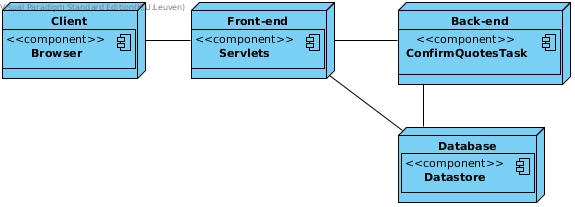
\includegraphics[width=\textwidth]{deployment-diagram.jpg}

\subsection{Sequence diagram}
See 'sequence-diagram.jpg'.

\section{GAE Exercise 3.3}
\subsection{Question 1}

Yes, such a scenario is plausible. We take the case in which there is only one queue and 2 workers as an example. When these workers are processing tasks in parallel and it just so happens that they both check the availability of a car at the same time, they will both assume the car is available. The system will then end up in an inconsistent state where two reservations are made for the same car for overlapping periods.

\subsection{Question 2}

One way to mitigate this problem would be to limit the amount of workers for the queue to just one. In this case there is an obvious trade-off between performance and consistency because of the lack of parallelism. We lose performance because tasks can no longer be processed in parallel, but we gain consistency because one confirmation of a quote is guaranteed to happen before the other in the scenario of Question 1. This approach is \textbf{not} scalable.

\subsection{Question 3}

Yes, in this case we can have one queue for each car rental company, each with a single worker.
Doing this allows for a certain degree of parallel processing again, as we can now process \texttt{confirmQuotesTasks} for different car rental companies in parallel.

\section{Note on back-channel}

After talking with the assistants during the practical sessions, we decided to use the GAE Mail API to realize a backchannel to the user. We chose this option because it's fairly easy to implement and it allows for a backchannel that doesn't actually require the user to visit the site to check the status of a task. This in essence makes it possible to \textbf{inform} the user of the task status, instead of letting the user \textbf{consult} the task status when he visits the site. \\\\
A confirmation mail is sent when the task is started, a second one is sent if the task fails or succeeds. Please note that the mail API just prints the mails to the console instead of sending them in while in development mode.

\end{document}
